\documentclass[Thesis.tex]{subfiles}
\begin{document}

\chapter{Surface panelization using periodic conformal maps}
\label{chp:periodic_conformal_maps}

This publication is joint work with Thilo R\"orig, Agata Kycia, and 
Moritz Fleischmann. It was previously published in the proceedings of the conference "Advances in Architectural Geometry 2014"~\cite{Roerig2014}.

\emph{Abstract:} 
We present a new method to obtain periodic conformal parameterizations of
surfaces with cylinder topology and describe applications to
architectural design and rationalization of surfaces. The method is
based on discrete conformal maps from the surface mesh to a cylinder or
cone of revolution. It comes with a number of degrees of freedom on
the boundary that can be used to obtain a variety of interesting
panelizations. We illustrate different choices of parameters for
\nurbs surface designs. Further, we describe how our parameterization
can be used to get a periodic boundary-aligned hex-mesh on a
doubly-curved surface. We optimize this initial mesh to consist of a
limited number of planar regular hexagons that panel the surface.

\begin{figure}
  \centering
  \includegraphics[width=0.49\textwidth]{images/teaser1_grid.pdf}
  \includegraphics[width=0.49\textwidth]{images/teaser2_2.pdf}
  \includegraphics[width=0.49\textwidth]{images/teaser4_1.pdf}
  \includegraphics[width=0.49\textwidth]{images/teaser3.pdf}
  \caption{For a cylindrical \nurbs surface (top-left) we create a
    seamless periodic conformal parameterization (top-right). A new
    mesh (bottom-left) is then rationalized and the panels are
    optimized for quantized regular hexagons (bottom-right).}
  \label{fig:teaser2}
\end{figure}

\def\subfilebibliography{}


\begin{figure}[tb]
\centering
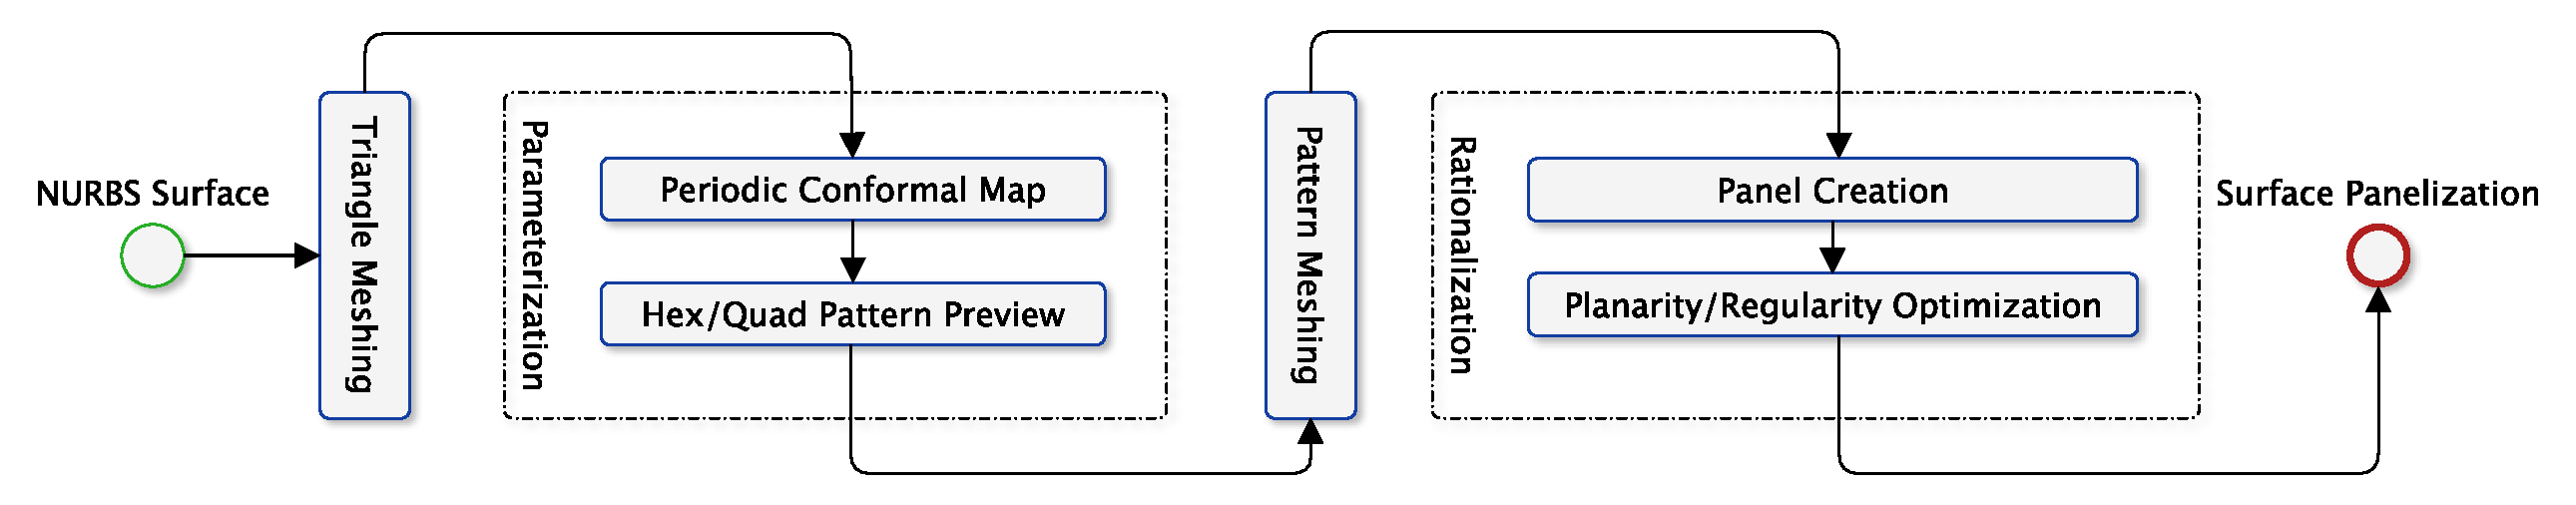
\includegraphics[width=\textwidth]{flowchart_bpmn_horizontal}
\caption{Flow diagram of the algorithms described in this paper. From
  a \nurbs surface a triangle mesh is created. The parameterization
  part is described in Section~\ref{sec:conformal-parameterization}. A
  pattern-mesh is created using this parameterization. The creation
  and optimization of panels is described in
  Section~\ref{sec:regular_hexagons}.}
\label{fig:algorithm_diagram}
\end{figure}

\section{Introduction}
\label{sec:introduction}

The panelization of surfaces remains a challenge in architectural
design. CAD software such as Rhino~\cite{rhino-website}, delivers powerful \nurbs surface
modelling to the designer. Their ease of use have made them a de facto
standard for the design of freeform (and other) shapes in
architectural design, especially envelopes and facades of buildings.  

The scale of buildings introduces challenges to surface-based
modelling strategies: The large scale of building elements demands
that they are divided into smaller elements. The cost of material and
labor, standardized production lines, green building concepts,
availability and redundancy during construction periods demands for a
high degree of similarity of these elements. Yet, the inherent
UV subdivision of \nurbs surfaces offers limited control over the
layout, shape and configuration of the panels. While strategies for
the controlled and careful creation of freeform surfaces have been
presented and realized~\cite{GlymphSCMS2004}, the tiling of true
freeform surfaces through alternative algorithms is still a challenge.

The quality of a surface panelization solution can be defined in
various ways. From an aesthetic point of view the shape of individual
elements is important. Further there are global conditions such as
alignment with surface boundaries and smooth transition of element
shape. From the standpoint of fabrication, the elements should be
repetitive. The contributions of this chapter are:

\begin{compactitem}[$\bullet$]
\item {\bf Periodic discrete conformal parameterization}:
  % 
  We present an algorithm that maps a triangle mesh with cylinder
  topology conformally to a cylinder or a cone of revolution. This
  allows us to obtain seamless patterns on surfaces. It is a
  generalized version of the discrete conformal parameterization
  scheme described by Springborn, Schr\"{o}der, and Pinkall~\cite{Springborn2008}.
\item {\bf Regular elements}:
  % 
  We show how the periodic discrete parameterization can be used to
  construct a panelization of the given periodic surface into a small
  number of repeating regular elements.
\item {\bf Applications to architectural design}: 
  % 
  We present a case study that initiated the development and where the
  described methods have successfully been applied in the architectural design
  context.
\end{compactitem}

The chapter is organized as follows:
Section~\ref{sec:parameterization} describes various parameterization
schemes available to architectural geometers. We briefly discuss the
shortcomings of current methods and explain how we adress them with our method.
Section~\ref{sec:conformal-parameterization} introduces the concept of
periodic discrete conformal parameterizations.  See
Figure~\ref{fig:algorithm_diagram} for a schematic view of the
proposed method. In Section~\ref{sec:panelization} we present a case
study that led to the development of this
work. Section~\ref{sec:regular_hexagons} deals with the optimization
of panels to meet requirements arising during the case study. We give
implementational details in Section~\ref{sec:implementation} and close
with an outlook on further research.

\section{Related work}
\label{sec:parameterization}

In this section we will review different methods used to
unroll/parameterize surfaces that are accessible in the architectural
design process on the example of Rhinoceros3D and 3rd party
plugins. All available tools lack at least one of the key features of
the proposed method:
\smallskip
\begin{compactitem}[$\bullet$]
\item \emph{Conformality} of the mapping avoids non-uniformly stretched
  panels
\item \emph{Periodicity} of the parameterization is needed to layout
  panels seamlessly on the surface
\item \emph{Boundary alignment} avoids irregular cutting of panels 
at the boundary of the surface  
\end{compactitem}

\begin{figure}[tb]
\centering
\includegraphics[width=0.32\textwidth]{images/failure-uv-marked.pdf}
\includegraphics[width=0.32\textwidth]{images/failure-squish-marked.pdf}
\includegraphics[width=0.32\textwidth]{images/failure-rectangle-marked.pdf}
\caption{State of the art unroll methods can create patterns on a
  closed surface.  The {\tt ApplyCrv} command of Rhinoceros produces
  boundary alinged periodic patterns but introduces unacceptable
  non-isotropic stretch (left). The {\tt SquishBack} method creates
  sufficiently regular elements but does not respect the periodicity
  of the surface (middle).  Non-periodic conformal maps align with the
  boundary of a cut surface. Along the cut the map is not continuous
  (right).}
\label{fig:failure}
\end{figure}

\subsubsection{Rhinoceros CreateUVCrv/ApplyCrv.}
A \nurbs surface is naturally equipped with a parameterization, i.e.,
a UV mapping from a rectangle domain to the surface. For the surface
of Figure~\ref{fig:teaser2} such a map can be used to project a pattern
from this rectangle to the surface ({\tt ApplyCrv} in Rhinoceros). The
pattern can be constructed periodically as it is defined in the UV
domain of the surface. However, in general this method does not
produce satisfactory results in terms of quality of elements for
complex freeform surfaces. The UV parameterization is not conformal
and thus introduces non-isotropic stretch and shear preventing the
elements to be regular on the surface, see Figure~\ref{fig:failure},
left. This limitation exists even for developable surfaces.

\subsubsection{Rhinoceros Squish/SquishBack.}
The {\tt Squish/SquishBack} command of Rhino maps a surface to the
plane minimizing the amount of stretch. While this is geometrically
not a conformal map it produces acceptable patterns on the surface. It
is however not capable of calculating periodic maps to the surface.
Thus it is not applicable in our situation, see
Figure~\ref{fig:failure}, middle.

\subsubsection{PanelingTools for Rhino.}
The paneling tools of Rhinoceros use the UV parameterization of the
underlying surface to populate grid-points over the surface. With the
help of such a grid, panels are placed onto the surface~\cite{panelingtools}. 
The shapes of the panels depend heavily on
the \nurbs-parameterization. An example is shown in
Figure~\ref{fig:failure}, left.

\subsubsection{Hexagonal tilings.}
In the architectural context, hexagonal panelizations have been
studied, e.g., by Zimmer~\emph{et~al.}~\cite{ZimmerCHK2013} and Troche~\cite{Troche2008}. 
These aproaches however do not include regularity or special boundary
alignment as introduced in the current work. In the work of 
Schiftner~\emph{et~al.}~\cite{SchiftnerHWP2009} the
result of the panelization depends on the choice of an initial
triangle mesh that is optimized towards touching incircles. This
allows for a torsion free support structure of a non planar
hex-mesh. Hexagonal tilings for triangulated surfaces also have been
studied by Nieser~\emph{et~al.}~\cite{NieserPPZ2012}. They focus on regularity but not on
boundary conditions.

\begin{figure}[tb]
\centering
\includegraphics[width=0.41\textwidth]{images/discrete_map_cylinder.pdf}
\reflectbox{\includegraphics[width=0.53\textwidth]{images/discrete_map_surface.pdf}}
\caption{A discrete periodic map from a cylinder to a triangulated
  surface.  On the cylinder all edges of the triangulation are
  geodesic arcs. If the cylinder is cut at the vertical orange path,
  then it can be unrolled to the plane creating a rectangular domain.}
\label{fig:discrete_map}
\end{figure}

\subsubsection{Mesh parameterizations.}
There are a vast number of parameterization schemes for meshes. To
elaborate on all methods is beyond the scope of this section and we
describe only the most relevant results here. General purpose
parameterization methods for triangle meshes produce high quality quad
or hex meshes for unstructured input 
data~\cite{BommesZK2009, AlexaCL2000, Springborn2008}. 
They have been used with success in the architectural context, e.g., by
 Bo~\emph{et~al.}~\cite{BoPKWW2011} and Sechelmann~\emph{et~al.}~\cite{Sechelmann2012}.

The basis of our method are conformally equivalent triangle meshes as
described by Springborn~\emph{et~al.}~\cite{Springborn2008}. The straight forward method to map a
surface with this approach is to cut it open and map it to a rectangle
domain. This method yields boundary aligned conformal maps that
however do not match along the introduced cut, see
Figure~\ref{fig:failure}, right. How to generalize this method to
overcome this limitation is the content of the following section.


\section{Periodic conformal parametrization}
\label{sec:conformal-parameterization}

\begin{figure}[tb]
  \centering
  \includegraphics[width=.28\linewidth]{images/conemap_aligned.pdf}
  \includegraphics[width=.32\linewidth]{images/conemap_singularities.pdf}
  \includegraphics[width=.37\linewidth]{images/conemap_isometric.pdf}
  \caption{Periodic domains of parameterization of the surfaces shown
    in Figure~\ref{fig:hex_example}.  Left: Map to a cylinder with
    geodesic boundary curves. Middle: Map to a cone of revolution with
    hex-pattern-adapted angle. The domain is a polygon with quantized
    angles. Right: Isometric boundary on a cone with
    hex-pattern-adapted angle.  Panelizations created with the help of
    these maps are shown in Figure~\ref{fig:hex_example}.}
  \label{fig:cone_maps_teaser}
\end{figure}

In this section we describe our algorithm for the creation of periodic
conformal maps for cylindrical meshes/surfaces, i.e., surfaces with
the same topology as a cylinder. First we will review the discrete
conformal maps of Springborn~\emph{et~al.}~\cite{Springborn2008}. Then we show how it can be generalized
to yield periodic maps to cylinders or cones.

A smooth \emph{conformal map} between two surfaces is a map that
preserves angles. Intuitively, one can think of a conformal map as a
map that preserves the shape but not the scale of small figures. For
conformal surface parameterization, one looks for conformal
maps from the plane to a surface and vice-versa. These can be used to 
map different patterns onto surfaces in a way that only isotropic
stretch/uniform scaling is applied to the pattern elements.
%
The method we build onto is a triangle mesh based
discretization of conformal maps~\cite{Springborn2008}. For each vertex~$v$ of
the surface -- interior or boundary -- we may prescribe an
angle~$\theta_v$ that corresponds to the angle sum of adjacent
triangles in the target mesh.  Starting from an input mesh and target
angles~$\theta_v$, the method calculates new edge lengths for the
triangles of the target mesh such that the angle sums at the target
vertices are as prescribed. This goal is achieved by minimizing a
convex functional.  
%
The prescribed angles have to satisfy a Gauss-Bonnet type condition,
i.e., the angles at interior vertices have to match the angles at the
boundary vertices.  We will state the condition for the special cases
treated later in the article, see Equation~\eqref{eq:theta}.

For the parameterization problem, we want to construct a map from a
surface to the plane. To get a planar target mesh, the target angles
have to be set to~$2\pi$ for all interior vertices, i.e., the angles
of the triangles adjacent to every interior vertex sum up
to~$2\pi$. Thus the computed target triangles can be laid out in the
plane. At the boundaries there is still a certain degree of freedom,
which allows to map the surface to different shapes, e.g., a rectangle
or a more general polygon with prescribed angles. 
%
An alternative choice of boundary conditions yields a target mesh
whose boundary edges have the same lengths as the original mesh. Then
the control over the boundary angles is no longer possible.

This method for the parameterization of triangle meshes can be generalized
to triangle meshes with cylinder topology, see Figure~\ref{fig:discrete_map}. 
Instead of constructing a discrete conformal map from the
surface to the plane, we construct a map to a cylinder or cone, whose image
is isometric to a polygonal region in the plane, see Figure~\ref{fig:cone_maps_teaser}. 
This works with an approach very similar to the previous one. We start 
with the definition of a periodic parameterization.

\begin{definition}
  Let~$M=(V,E,F)$ be a mesh with cylinder topology and vertices~$V$,
  edges~$E$, and triangles~$F$. Let~$D\subset C$ be a region on a
  cone/cylinder of revolution.  A continuous bijection $\Phi:D\to M$
  is called a \emph{discrete periodic parameterization}. $D$ is called
  the \emph{domain of parameterization}.
\end{definition}

In the latter we always assume that the preimages of edges of $M$ are geodesic 
arcs on the cone/cylinder $C$.
For panelization of periodic surfaces we need to make sure, that
different patterns match around the cone or cylinder. This yields
certain restrictions on the cone that serves as domain of parameterization.

\noindent
\begin{minipage}{0.55\linewidth}
  \begin{definition}
    Let~$C$ be a cone with aperture~$\varphi$ and~$\Phi:C\supset D\to M$ be a
    discrete periodic parameterization of a triangle mesh~$M$ with domain~$D$. 
    The map $\Phi$ is called \emph{triangle adapted} if the cone angle $\alpha$ is 
    a multiple of $\frac{\pi}{3}$ and \emph{quad-pattern adapted} if it is a
    multiple of $\frac{\pi}{2}$.
  \end{definition}
\end{minipage}
\begin{minipage}{0.4\linewidth}
  \centering
  \begin{overpic}[height=4cm]{images/cone_angle.pdf}
    \put(38,78){\footnotesize$\varphi$}
    \put(50,60){\footnotesize$1$}
    \put(37,33){\footnotesize$\sin(\varphi/2)$}
    \put(10,10){\footnotesize$\alpha = 2 \pi \sin(\varphi/2)$}
  \end{overpic}
\end{minipage}

This definition ensures that either a quad-, triangle-, or hex-pattern 
fits seamlessly onto the surface after parameterization.


\begin{figure}[p]
  \centering
  \includegraphics[width=.89\textwidth]{images/quantized_aligned5.pdf}
  \includegraphics[width=.89\textwidth]{images/quantized_singularities5.pdf}
  \includegraphics[width=.89\textwidth]{images/quantized_isometric2.pdf}
  \caption{Quantized periodic hexagonal panelizations. Boundary
    conditions affect the amount of stretch in the interior of the
    surface. Top: Hexagonal pattern aligns with the boundary, a strong
    condition that produces large deviation of panel sizes. Middle:
    Map to a pattern-adapted polygon on a cone of revolution. The
    pattern contains exceptional points at the boundary. The stretch
    is minimized while at the same time the pattern alignes with the
    boundary.  Bottom: Conformal map with the least stretch in the
    interior, pattern can be optimized to consist of congruent
    hexagons alone. In each image, panels with the same colors are
    congruent. The corresponding domains of parameterization are shown
    in Figure~\ref{fig:cone_maps_teaser}.}
  \label{fig:hex_example}
\end{figure}

\subsection{Periodic boundary conditions}
\label{sec:boundary}

If we want to construct periodic conformal maps we are allowed
to specify angle sums~$\theta_v$ at boundary vertices. The condition
for the sums of boundary angles differs from the simply-connected case in the
following way: The curvature at a boundary vertex~$v$ is given by
$\kappa_v = \pi -\theta_v$, where $\theta_v$ is the angle sum of the
adjacent triangles in the target mesh. For the two boundary loops
$(v_1, \ldots, v_n)$ and $(w_1, \ldots, w_m)$ we have:
\begin{equation}
\sum_{i=1}^n \kappa_{v_i} + \sum_{j=1}^m \kappa_{w_j} = 0. \label{eq:theta}
\end{equation}
This condition makes sure that the two boundary curves ``bend'' the
same amount and can hence be wrapped around a cone. 
We will now show how boundary conditions can be
used to construct periodic patterns on the studied models. We start
with a discrete conformal map of the doubly-curved model from Figure~\ref{fig:teaser2} 
to a standard cylinder. 

\subsubsection{Straight cylinder.}
The simplest way to generate a map to the cylinder is to set the
target angles for all boundary vertices to~$\pi$. Hence the curvatures
at the boundary vertices are zero and the two boundary loops are
mapped to ``straight'' curves. 
In this case both angle sums of Equation~\eqref{eq:theta}
vanish and the target mesh can be wrapped around a cylinder, see 
Figure~\ref{fig:cone_maps_teaser}, left. The new edge lengths
computed with the variational principle correspond to the lengths on a
cylinder. This cylinder can be unrolled into the plane preserving angles
and lengths. Therefore the two boundary polygons are mapped to straight lines
in the plane. These two straight lines have to be parallel and of
equal lengths.
%
If the lengths of the boundary curves in the original model differ a
lot, then a map to a cylinder induces a lot of conformal stretch. This stretch
can be reduced by specifying special boundary conditions for a
parameterization on a cone of revolution.

\subsubsection{Cone of revolution.}
As long as Equation~\eqref{eq:theta} is satisfied we obtain a map to a
general cone of revolution. In our case, we require that the
periodic parameterization is adapted to the target pattern. 
This means that the two sums of Equation~\eqref{eq:theta} need to 
be (the same) multiples of
$\tfrac{\pi}{3}$ (triangle or hex) or multiples of $\tfrac{\pi}{2}$
(quad). We present two methods to achieve this requirement: a uniform
distribution and a concentration of curvature.

If the boundary of the mesh should align with the pattern,
then boundary angles need to be quantized, i.e., multiples of
$\tfrac{\pi}{3}$ or~$\tfrac{\pi}{2}$ need to be chosen as target
angles. In Figure~\ref{fig:cone_maps_teaser}, middle, three vertices
of the top and bottom boundary curve were manually assigned to
$\tfrac{4}{3}\pi$ and~$\tfrac{2}{3}\pi$, respectively. All other
boundary angles are set to~$\pi$, i.e., straight.  Such a map can
be used as a starting point to obtain a tesselation with quantized
hexagons as described in Section~\ref{sec:regular_hexagons}.

It is known that a discrete confomal map that does not change the lengths of the 
boundary edges exhibits the least stretch in the interior of the surface.
To obtain such a parameterization we first construct a periodic conformal 
mapping onto an
arbitrary cone such that the lengths of the boundary edges are equal. The resulting angle sums at boundary vertices of the
target mesh determine the cone angle~$\varphi$ of the map. The cone angle of
a pattern adapted periodic parameterization is the closest multiple of the 
desired quantization. We distribute the difference to the closest
quantized angle uniformly to the individual boundary vertices and
recompute the map with these angle conditions. The obtained map is 
periodic and exhibits the lowest stretch of all periodic conformal maps (see
Figure~\ref{fig:cone_maps_teaser}, right).  

\begin{figure}[bt]
  \centering
  \includegraphics[width=.52\linewidth]{images/wanda_entrances2.pdf}
  \hspace{.5cm}
  \includegraphics[width=.32\linewidth]{images/wanda_diagrid2.pdf}
  \caption{A periodic conformal map onto a cylinder with special
    vertices creates the opportunity to incorporate entrances (left)
    or concentration of support structure (right).}
  \label{fig:entrance}
\end{figure}

\subsubsection{Design and structural opportunities.}
Opposed to achieving a homogenous pattern distribution, as described
previously, it is also possible to use special boundary conditions to
support structural purposes or design requirements. If one aims for a
panelization with boundary aligned patterns, then the target boundary
angles must be quantized.

To include entrances in a facade it is possible to incorporate special 
boundary conditions. An example with special boundary vertices with domain angles
$\frac{4}{3}\pi$ and $\tfrac{\pi}{3}$ is shown in
Figure~\ref{fig:entrance}, left. In the remeshed surface, the lower boundary
curve bends inside at the vertices with angle~$\tfrac{4}{3}\pi$ around
the vertex with angle~$\tfrac{\pi}{3}$. This incorporates a natural
entrance into the facade.

Another effect of such angle conditions is a densification of the
pattern at the vertices with small angles. Such a concentration of
elements can be used to enforce structural properties of a
geometry. An example of a diagrid generated with such boundary
conditions is shown in Figure~\ref{fig:entrance}, right.


\section{Case study: Hexagonal surface panelization}
\label{sec:panelization}
Here we present the findings of a first case study, where the method
of discrete conformal mappings was utilized for a real-world project.
In this case study, a facade design, important questions concerning
panel layout, similarity and therewith constructability had to be
addressed at the early design stage.

Discrete conformal maps were used, as they allow the designer to
explore alternative surface textures and surface panelizations with
great design flexibility. This distinguishes the method from more
constrained modelling techniques~\cite{GlymphSCMS2004}. Through the method of
conformal mapping, opposed to naive UV mapping, the density of the
surface panelization varies across the entire surface, yet the shape
of elements does not. This can be used for structural purposes, such
as diagrid layouts, or design driven, such as window distribution, see 
Figure~\ref{fig:entrance}. The optimization of the surface panelization 
towards multiple criteria such as edge length and planarity was 
consequential.

\begin{figure}[t]
  \centering
  \includegraphics[width=0.93\textwidth]{images/henn/overview02.pdf}
  \caption{Rendering of Case Study - A project where the method of
    conformal mapping was utilized for the facade design.}
  \label{fig:overview02}
\end{figure}

For a commissioned competition entry we tested and developed the
method of periodic conformal mappings. The project, which served as a
case study, was highly constrained, as the architects were asked to
propose an alternative facade design for an existing design proposal
of a multifunctional exhibition center in China, see
Figure~\ref{fig:overview02}. The massing was fixed, but there were 2
alternative massing options (1 single curved and 1 doubly-curved
envelope) to be explored. Also, the client wanted a hexagonal tiling
on the facade but only had a very limited budget of approximately 200
Euro / sqm for the entire facade including sub structure in mind.

These limitations, in combination with the very short timeframe of 2
weeks for the entire redevelopment of the facade including a
feasibility study drove the development of the conformal mapping
method. Especially, since existing solutions such as UV mapping led to
unsatisfactory results producing anisotropic stretch and shear of some
regions in the master surfaces.  Some specific questions that had to
be addressed for each massing option were:
\smallskip
\begin{compactitem}[$\bullet$]
\item How many (different) panels would we need?
\item Can we clad the entire surface with planar tiles?
\item Can we equalize the edge lengths of each hexagon?
\item Can we control the orientation of the panels?
\item Can we achieve a regular pattern with a homogeneous visual
  appearance?
\end{compactitem}
\smallskip
In the end, all the above questions were answered/solved.

The first step of development focused on achieving periodicity across
the surface and alignment with the boundary. While the issue of
periodicity directly addressed the last question, it is strongly
related to the others as they could be achieved by successive
optimization steps.

\begin{figure}[t]
  \centering
  \includegraphics[width=0.93\textwidth]{images/henn/panel_construction.pdf}
  \caption{The data for the component-like construction of each panel was derived from the mesh.}
  \label{fig:panel_construction}
\end{figure}

Already during the design phase a fully periodic tiling was
achieved. In a following step the panels were planarized, grouped by
dimension and their edge lengths were equalized. Finally, a control
for the panel orientation based on the tangents of the \nurbs master
surface was implemented. This hexagonal pattern served as a base for
the facade engineering team. Due to the high cost demands, a simple
component system that served as a sub-structure for each panel was
developed, see Figure~\ref{fig:panel_construction}.

Unfortunately the given massing options for the building were not very
challenging in terms of geometry. One massing option was a simple
extrusion and the other had very little distortion. After the
successful submission of the project, we decided to continue the
development and test the method of discrete conformal mappings on more
extreme base geometries.

During these tests a Grasshopper plug-in for \VaryLab has been developed 
and refined~\cite{varylab-web-page}. We focused
on tiling surfaces with a large distortion/stretch and double
curvature. The main aim was to tile these surfaces without
distorsion. This led to focus on the boundary conditions. The designer
is now able to choose between an aligned mapping where the tile-pattern
aligns with the underlying surface boundary. The trade-off being, that
panels need to vary in sizes. Or one chooses a ``homogeneous tiling'',
where all the tiles are the same, but do not align with the
boundary. \VaryLab's numerous optimization algorithms can be applied
and combined with either of the two approaches, see
Figure~\ref{fig:hex_example}. During the development, we realized that
through singularities and special boundary conditions, one is able to
control the density and distribution of the pattern on the surface and
along its boundaries, see Figure~\ref{fig:entrance}.

\begin{figure}[bt]
  \centering
  \includegraphics[width=0.93\textwidth]{images/henn/detail.pdf}
  \caption{Close-up rendering of facade.}
  \label{fig:detail}
\end{figure}


\newcommand{\Ealpha}{E_\alpha}
\newcommand{\Eedge}{E_\ell}

\section{Rationalization: Hexagon optimization}
\label{sec:regular_hexagons}

Starting from the conformal parameterization we optimize the obtained
hex-mesh to have identical regular hexagons. We use a global
optimization approach and define energies to achieve \emph{planarity},
\emph{regularity}, and \emph{equality}.

\subsubsection{Planarity.} 
The planarity function is a simple adaptation of the usual energy used
to planarize quad-meshes: A quadrilateral $\{A, B, C, D\}$ is planar
if the volume of the tetrahedron $\{A, B, C, D\}$ is zero. So if we
require the volume of all tetrahedra spanned by the vertices of a polygon
to be zero we obtain a planar polygon.  The planarity energy~$\Epl$
can easily be expressed in terms of determinants.

\subsubsection{Regularity.}
A regular planar polygon is characterized by having equal edge lengths
and equal angles at all vertices. As for planarity we define an energy
that is minimized in case of regular polygons. The interior angle at a
vertex of a regular $p$-gon is $\tfrac{p-2}{p} \pi$. So an energy $\Ereg$
that is minimized for a regular $p$-gon with vertices $\{v_1, \ldots,
v_p\}$ and corresponding angles $\{\alpha_1, \ldots, \alpha_p\}$ is
\begin{align*}
\Ereg(P) &= \lambda_P\  \Ealpha(P) + \mu_P\ \Eedge(P) &&\text{with}\\ 
\Ealpha(P) &= \sum_{i=1}^p (\alpha_i - \frac{p-2}{p} \pi)^2 
&& \Eedge(P) = \sum_{(v_i,v_{i+1})} (\|v_i - v_{i+1}\| - \ell_P)^2,
\end{align*}
where $\ell_P$ is the desired target edge length for the polygon and
$\lambda_P$ and~$\mu_P$ weights for the different energies. In a first
step, the target length can be chosen to be the average edge length of
the polygon or the shortest edge length among the edges to avoid
overlap.  Note that, the normalization of the angles already implies
planarity of the polygons.  Nevertheless, we consider the planarity
energy since it increases the rate of convergence.

Starting from a cylindrical or conical periodic conformal
parameterization we construct a hex-mesh that may or may not be
aligned with the boundary. As a consequence of the conformality of the
parameterization the angles of the hexagons are almost
$\tfrac{2\pi}{3}$. In the following we do not work with a water tight
mesh any more but split the surface into individual hexagonal
panels. We optimize the edge lengths of the hexagons to be constant
per face using~$\Eedge$. To avoid overlap we choose the length of the
shortest edge of each face as target length. We add the planarity and
angle regularity functionals~$\Epl$ and~$\Ealpha$ to the optimization
and obtain planar and regular hexagons. Each of the hexagons has its
own constant edge length. Finally, we can rationalize the panelization
further, by choosing a discrete set of edge lengths as target lengths
for the polygons in the edge length functional~$\Eedge$. Due to the
symmetry of the edge length functional for regular hexagons edge
length optimization will not destroy the planarity and regularity of
the hexagons. So it is possible to adjust the edge lengths
using~$\Eedge$ only. This quantization process is illustrated in
Figure~\ref{fig:quantization}.
%
The used method allows to include additional functionals into the
optimization, e.g., functionals minimizing the distance to a reference
surface or the distribution of gaps tangent and normal to the
surface. We have not yet added these functionals due to the early
phase of the presented project.


\begin{figure}[tbp]
  \centering
  \includegraphics[width=0.48\textwidth]{images/wanda_curved_unquantized.pdf}
  \includegraphics[width=0.48\textwidth]{images/wanda_curved_quantized.pdf}
  \caption{Panelization of a doubly curved design alternative of the
    case study shown in Figure~\ref{fig:overview02}. Left: Unquantized
    panelization.  Right: Quantization to $11$ panel sizes with edge
    lengths varying from 1.5m to 2m.}
  \label{fig:quantization}
\end{figure}

The range of lengths obtained depends on the initial hex-mesh
constructed on the chosen target geometry. The effect of the
different periodic conformal parameterizations on the quantization is
shown in Figures~\ref{fig:cone_maps_teaser} and~\ref{fig:hex_example}.


\section{Implementation}
\label{sec:implementation}

We use the software package \VaryLab~\cite{varylab-web-page} in
combination with Rhino's Grasshopper to calculate discrete conformal
maps to the cylinder or cone as shown in Figure~\ref{fig:cone_maps_teaser}.
Figure~\ref{fig:grasshopper} shows the Grasshopper network used to
connect Rhino and \VaryLab.
\VaryLab uses the optimization package {\sc TAO/PETSc}~\cite{tao-user-ref, 
petsc-web-page, jpetsctao-web-page} to perform energy
minimization.
%
We calculated the exact gradients of the functionals for the
optimization and used the conjugate gradient method of {\sc TAO}.

\begin{figure}[tb]
	\includegraphics[width=0.47\textwidth]{images/setup03_neu.pdf}
	\hspace{0.06\textwidth}
	\includegraphics[width=0.47\textwidth]{images/setup04_neu.pdf}
	\caption{Grasshopper networks connecting Rhino and
          \VaryLab{}. In the first step we send mesh data to \VaryLab{}
          running on the same machine at {\tt localhost:6789}
          (left). In the second step we collect the result from this
          \VaryLab{} instance and create polygons from the mesh's
          faces (right).}
	\label{fig:grasshopper}
\end{figure}


\section{Conclusion}
\label{sec:conclusion}

The collaboration between architect and math department proved to be
very satisfactory for both parties: The architects did provide
specific questions related to real world projects whilst the
mathematicians were able to translate these questions into
mathematical formulas and provided meaningful results that could not
have been achieved alternatively. A common design framework such as Rhino
and the basic knowledge of \nurbs geometry and modeling techniques
proved to be of essential importance for the successful collaboration
between the teams.

As a result of this collaboration, we presented a method for
homogeneous periodic panelization of \nurbs surface geometry of
cylinder type.  A natural future development is the design of suitable
support structures possibly with torsion free nodes. This can be
derived from the panel layout by intersecting the panel
planes. Furthermore the quantization of edge lengths of regular
hexagonal panels is not yet fully explored. A denser distribution of
quantized edge lengths in regions with great edge length variance can
possibly improve the layout and number of different panels. 
%
For a later stage of the project one could add optimization for the
gaps between the panels, which has not been incorporated yet. It would
also be interesting to look at more extreme examples, even if those
might not fit the architectural context.

We also started to look into how patterns can be applied across
multiple surface patches, such that the pattern aligns at the crease
where the patches meet. This would necessitate to develop methods for
more general mappings and the applications of multiple boundary
conditions; A field that is yet to be developed.

While the method presented does require a certain level of expertise
from the user, we see the potential of this post-panelization strategy
of freeform surfaces in the architectural design process: Opposed to
carefully constrained (parametric) modelling approaches this method
allows to realize even distributed, homogenous panelizations on
arbitrary surfaces with cylinder topology at early design stages -
something a lot of designers are interested in.

%\subfile{publications/AAG2014-Periodic/final/introduction.tex}
%\subfile{publications/AAG2014-Periodic/final/parametrization.tex}
%\subfile{publications/AAG2014-Periodic/final/conformal-parametrization.tex}
%\subfile{publications/AAG2014-Periodic/final/boundary-conditions.tex}
%\subfile{publications/AAG2014-Periodic/final/panelization.tex}
%\subfile{publications/AAG2014-Periodic/final/hexagons.tex}
%\subfile{publications/AAG2014-Periodic/final/implementation.tex}
%\subfile{publications/AAG2014-Periodic/final/conclusion.tex}

\subfilebibliographytwo
\end{document}

%%% Local Variables:
%%% TeX-master: "Thesis.tex"
%%% End: